%%% template.tex
%%%
%%% This LaTeX source document can be used as the basis for your technical
%%% paper or abstract. Intentionally stripped of annotation, the parameters
%%% and commands should be adjusted for your particular paper - title, 
%%% author, article DOI, etc.
%%% The accompanying ``template.annotated.tex'' provides copious annotation
%%% for the commands and parameters found in the source document. (The code
%%% is identical in ``template.tex'' and ``template.annotated.tex.'')

\documentclass[conference]{acmsiggraph}

\TOGonlineid{45678}
\TOGvolume{0}
\TOGnumber{0}
\TOGarticleDOI{1111111.2222222}
\TOGprojectURL{}
\TOGvideoURL{}
\TOGdataURL{}
\TOGcodeURL{}

\title{The Title of Your Paper Goes Here}

\author{Yanling He\thanks{e-mail:heyl@cs.washington.edu}\\Computer Science \& Engineering\\University of Washington
\and
Xin Yang\thanks{e-mail:yx1992@cs.washington.edu}\\Computer Science \& Engineering\\University of Washington
\and
Xiaoyi Zhang\thanks{e-mail:xiaoyiz@cs.washington.edu}\\Computer Science \& Engineering\\University of Washington
}
\pdfauthor{Yanling He}
\pdfauthor{Xin Yang}
\pdfauthor{Xiaoyi Zhang}

\keywords{radiosity, global illumination, constant time}

\begin{document}

%% \teaser{
%%   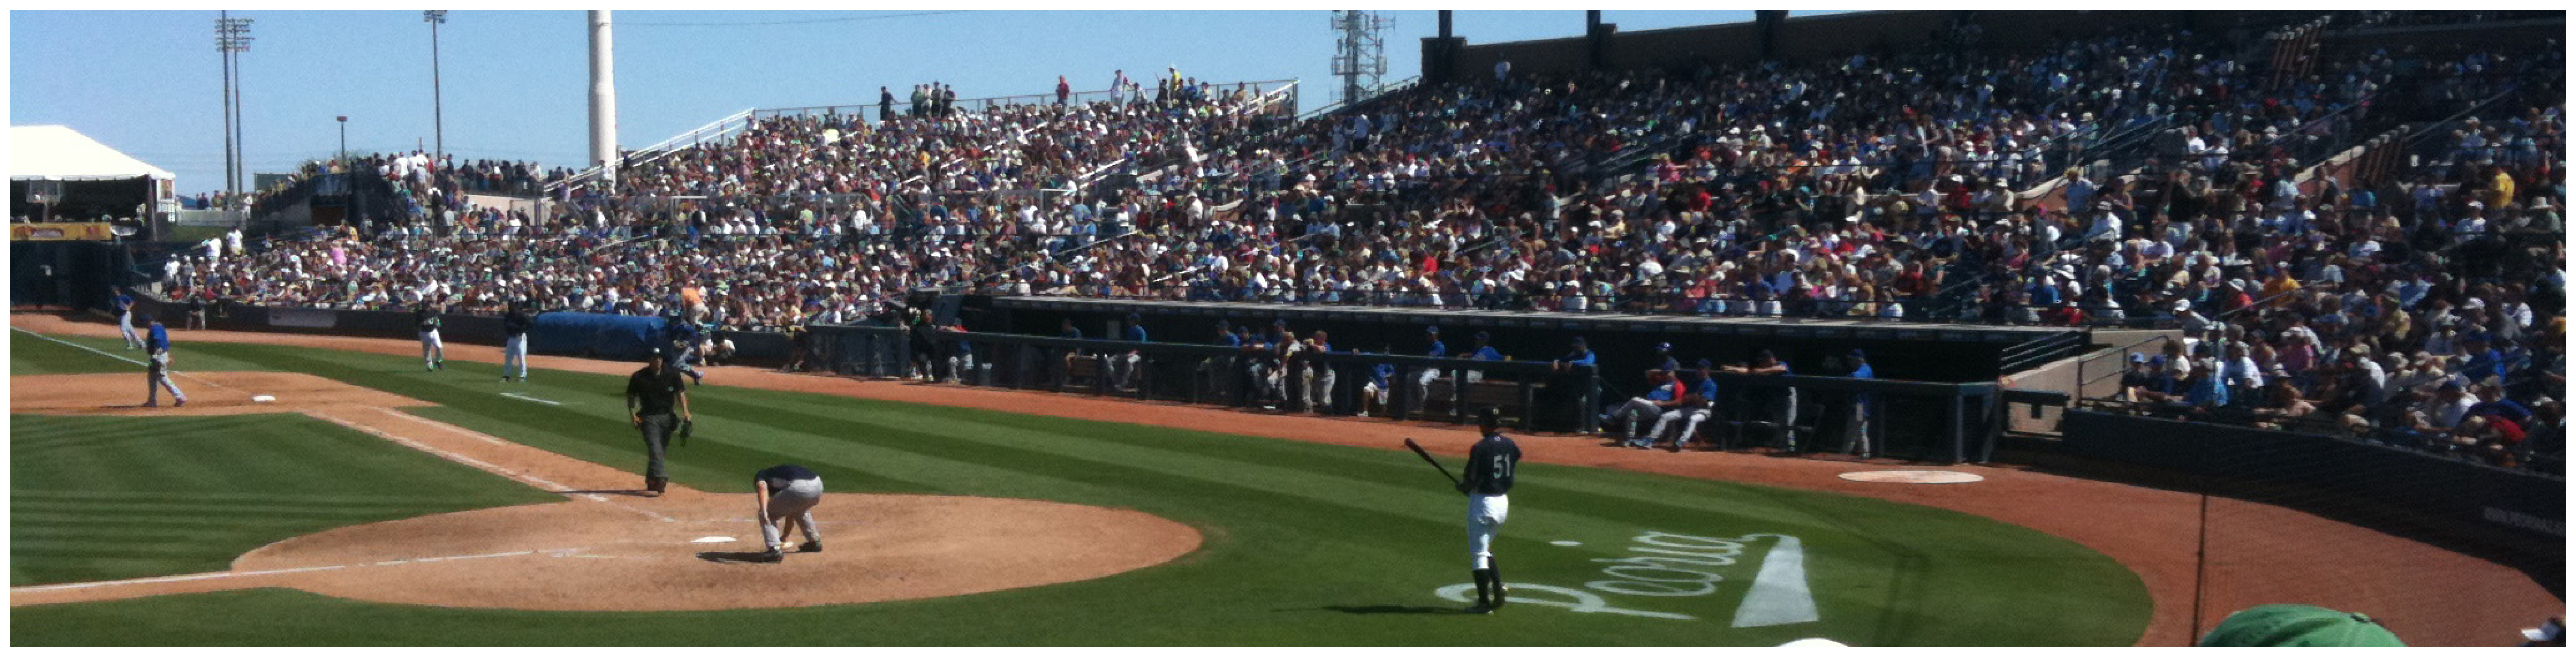
\includegraphics[height=1.5in]{images/sampleteaser}
%%   \caption{Spring Training 2009, Peoria, AZ.}
%% }

\maketitle

\begin{abstract}

This project analyzes the relationship of Instagram filter data with location, number of likes and hashtag to give users filter suggestion on achieving more likes based on users' location and the photo content, and analyzes visual culture differences between the cities. It shows three types of data relationship: first, filter usage based on different cities; second, in each city the number of likes of each filter; third, in each city what hashtag are labeled most.

\end{abstract}

\begin{CRcatlist}
  \CRcat{I.3.3}{Computer Graphics}{Three-Dimensional Graphics and Realism}{Display Algorithms}
  \CRcat{I.3.7}{Computer Graphics}{Three-Dimensional Graphics and Realism}{Radiosity};
\end{CRcatlist}

\keywordlist

%% Use this only if you're preparing a technical paper to be published in the 
%% ACM 'Transactions on Graphics' journal.

\TOGlinkslist

%% Required for all content. 

\copyrightspace

\section{Introduction}

You may have ever scrolled through the Instagram filter list back and force worrying about which one to use, and how to make more people like it. But since culture background and contents varies a lot from photo to photo, it is hard to make a simple suggestion that let everyone like it. To solve this problem our project analyzes the Instagram filter data based on location, likes and hashtag.

This project analyzes how filter usage are distributed in 50 cities, which are the cities with most population in each state of United States, and it also shows the number of likes for each filter. This shows the filter preference and how culture varies at different places. It also analyzes the number of hashtags been labeled on the posts for each city. 

The goal of this project is to give useful filter suggestion and showing visual culture and content differences for different states. 

\section{Related Work}

Citations can be done this way~\cite{Jobs95} or this more concise 
way~\shortcite{Jobs95}, depending upon the application.

Lorem ipsum dolor sit amet, consectetur adipisicing elit, sed do
eiusmod tempor incididunt ut labore et dolore magna aliqua. Ut enim ad
minim veniam, quis nostrud exercitation ullamco laboris nisi ut
aliquip ex ea commodo consequat. Duis aute irure dolor in
reprehenderit in voluptate velit esse cillum dolore eu fugiat nulla
pariatur. Excepteur sint occaecat cupidatat non proident, sunt in
culpa qui officia deserunt mollit anim id est laborum.

\section{Methods}

Lorem ipsum dolor sit amet, consectetur adipisicing elit, sed do
eiusmod tempor incididunt ut labore et dolore magna aliqua. Ut enim ad
minim veniam, quis nostrud exercitation ullamco laboris nisi ut
aliquip ex ea commodo consequat. Duis aute irure dolor in
reprehenderit in voluptate velit esse cillum dolore eu fugiat nulla
pariatur. Excepteur sint occaecat cupidatat non proident, sunt in
culpa qui officia deserunt mollit anim id est laborum.

\begin{figure}[ht]
  \centering
  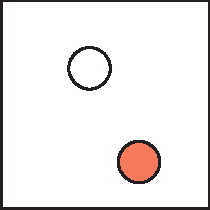
\includegraphics[width=1.5in]{images/samplefigure}
  \caption{Sample illustration.}
\end{figure}
Lorem ipsum dolor sit amet, consectetur adipisicing elit, sed do
eiusmod tempor incididunt ut labore et dolore magna aliqua. Ut enim ad
minim veniam, quis nostrud exercitation ullamco laboris nisi ut
aliquip ex ea commodo consequat. Duis aute irure dolor in
reprehenderit in voluptate velit esse cillum dolore eu fugiat nulla
pariatur. Excepteur sint occaecat cupidatat non proident, sunt in
culpa qui officia deserunt mollit anim id est laborum.

\section{Future Work}

\subsection{Computer Vision Analysis}
Since not all the photos are labeled with hashtags and not all the hashtags are correctly showing the content in each photo, using computer vision to analysis the real photo content, the style of the scenes and the major color theme may have stronger correlation with the filter types.
\subsection{Relationship with Time}
As the time changes people’s vision preference may also changes, so the preference of filters may shifts as the time changes, we can learn the relationship with filters, likes and time to learn how visual preference changes and give out more current filter suggestion.
\subsection{World Map}
Since all the location analysis are based on the United States, so culture variety may be less between each cities, to extend the data to world based to learn some culture different between continents may give us more meaningful data. But world-wise spread of the Instagram usage may be the limit of this extension.

\section{Conclusion}

Lorem ipsum dolor sit amet, consectetur adipisicing elit, sed do
eiusmod tempor incididunt ut labore et dolore magna aliqua. Ut enim ad
minim veniam, quis nostrud exercitation ullamco laboris nisi ut
aliquip ex ea commodo consequat. Duis aute irure dolor in
reprehenderit in voluptate velit esse cillum dolore eu fugiat nulla
pariatur. Excepteur sint occaecat cupidatat non proident, sunt in
culpa qui officia deserunt mollit anim id est laborum.

\section*{Acknowledgements}

To Robert, for all the bagels.

\bibliographystyle{acmsiggraph}
\bibliography{template}
\end{document}
